Dieses Kapitel  behandelt in Kurzform  die wichtigsten Grundlagen,  welche zum
Verst\"andnis des Versuches erforderlich sind.

% **************************************************************************** %
\subsection{Grundidee}
\label{sec:arbgru:subsec:grundidee}
% **************************************************************************** %

Wird ein Wechselstrom durch einen  Leiter \"ubertragen, so ist die Stromdichte
im Leiter  nicht gleichf\"ormig.   Hochfrequente Str\"ome  (oder hochfrequente
Stromanteile, bei einer \"Uberlagerung harmonischer Schwingungen verschiedener
Frequenzen) weisen  im Inneren  des Leiters  eine niedrigere  Stromdichte auf,
als  im  \"ausseren Bereich. Es  werden  im  Leiter Wirbelst\r"ome  induziert,
welche hochfrequente  elektromagnetische Felder  gegen das Innere  des Leiters
abschirmen.

In  diesem   Versuch  soll  dieses  Verhalten   (auch  als  \emph{Skinneffekt}
bezeichnet)  anhand einer  stromdurchflossenen Spule  mittels Einf\"uhren  von
Hohlzylindern und Vollzylindern  untersucht werden, wobei dabei  das B-Feld im
Innern der Spule gemessen wird und dabei R\"uckschl\"usse auf den Spulenstrom
gemacht werden.


% **************************************************************************** %
\subsection{Vollzylinder}
\label{sec:arbgru:subsec:vollzylinder}
% **************************************************************************** %

Es sollen in  diesem Abschnitt kurz die wichtigsten  Zusammenh\"ange f\"ur den
Fall des Vollzylinders aufgef\"uhrt werden.

% ---------------------------------------------------------------------------- %
\subsubsection{DGL f\"ur das B-Feld}
\label{sec:arbgru:subsec:vollzylinder:herleitDGL}
% ---------------------------------------------------------------------------- %


\begin{figure}[th!]
    \centering
    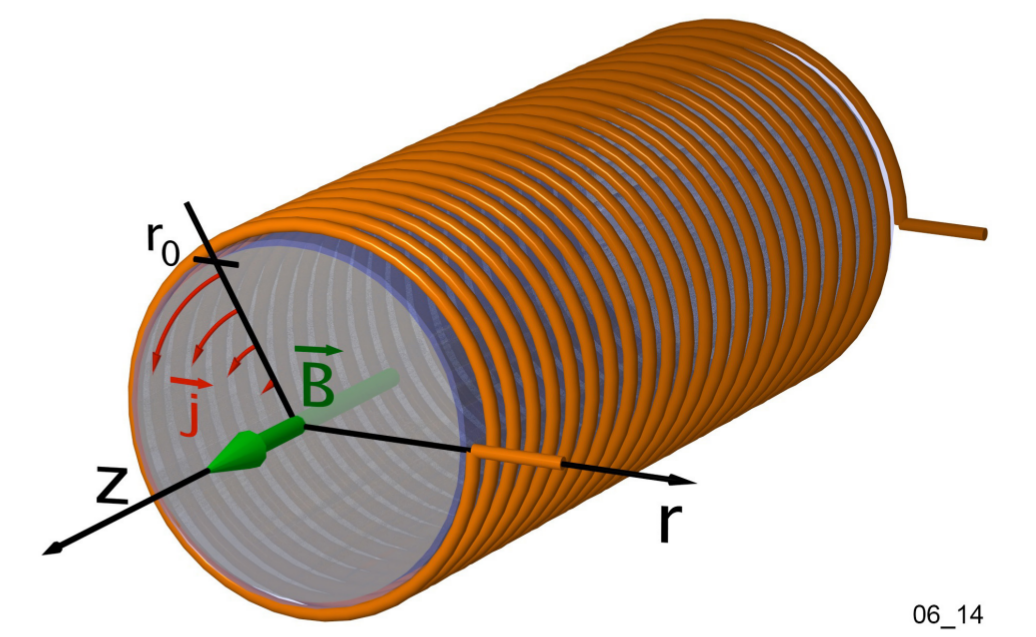
\includegraphics[width=.5\textwidth]{images/spule-vollzylinder.png}
    \caption{Spule mit Vollzylinder \emph{Quelle:} Skript zum Versuch}
\end{figure}


% ---------------------------------------------------------------------------- %
\subsubsection{B-Feld, exakte L\"osung}
\label{sec:arbgru:subsec:vollzylinder:bFeldexakt}
% ---------------------------------------------------------------------------- %


% ---------------------------------------------------------------------------- %
\subsubsection{Selbstinduktionskoeffizient und Ohm'scher Widerstand, exakte L\"osung}
\label{sec:arbgru:subsec:vollzylinder:LRexakt}
% ---------------------------------------------------------------------------- %


% **************************************************************************** %
\subsection{Hohlzylinder}
\label{sec:arbgru:subsec:hohlzyliner}
% **************************************************************************** %

Es sollen in  diesem Abschnitt kurz die wichtigsten  Zusammenh\"ange f\"ur den
Fall des Hohlzylinder aufgef\"uhrt werden.

% ---------------------------------------------------------------------------- %
\subsubsection{B-Feld}
\label{sec:arbgru:subsec:vollzylinder:herleitDGL}
% ---------------------------------------------------------------------------- %


\begin{figure}[th!]
    \centering
    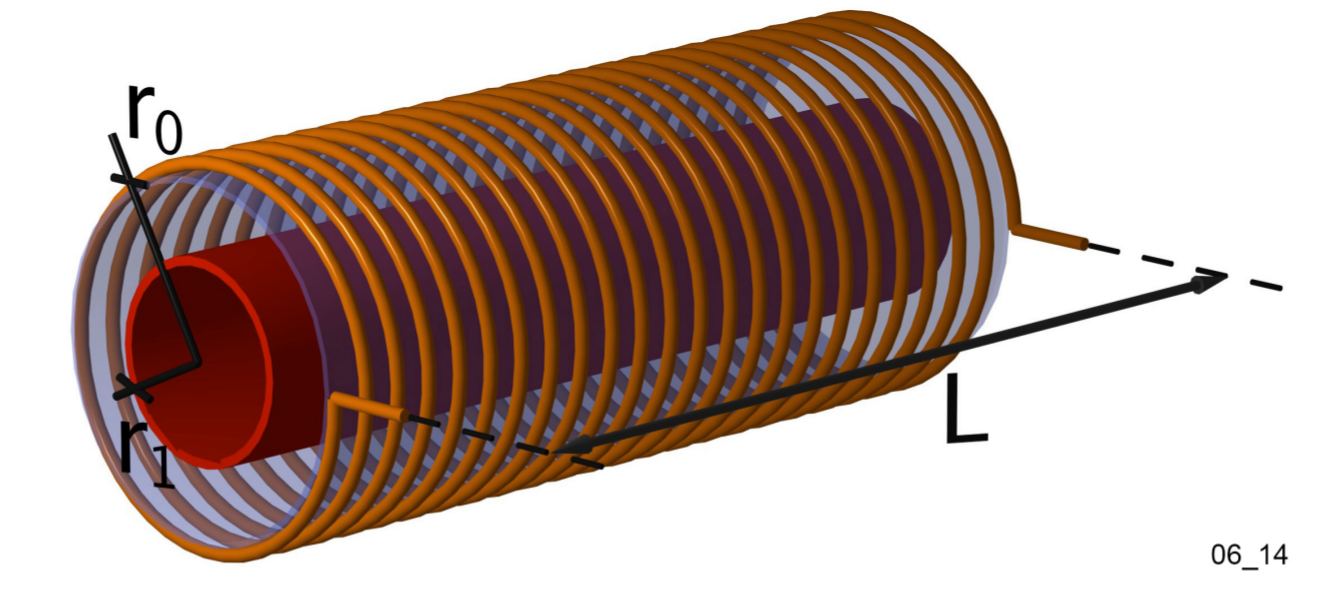
\includegraphics[width=.5\textwidth]{images/spule-hohlzylinder.png}
    \caption{Spule mit Hohlzylinder \emph{Quelle:} Skript zum Versuch}
\end{figure}



% ---------------------------------------------------------------------------- %
\subsubsection{Selbstinduktionskoeffizient und Ohm'scher Widerstand, exakte L\"osung}
\label{sec:arbgru:subsec:vollzylinder:LRexakt}
% ---------------------------------------------------------------------------- %
